%\documentclass[convert]{standalone}
\documentclass{article}
\usepackage[margin=0.1in]{geometry}

\usepackage[table]{xcolor}
\usepackage{amsmath, graphics}
\usepackage[makeroom]{cancel}
\usepackage{fdsymbol}
\usepackage{adjustbox}
\newcommand{\co}[1]{{\color{red}CO~#1}}
\begin{document}



\pagestyle{empty}
\begin{table}[h!]
\centering
\rowcolors{1}{gray!50}{white}
\begin{adjustbox}{width=\textwidth}
\begin{tabular}{|c | c  | l | l| }
	\hline
	&     &                              & PHYS                                           \\
	20 fall  & 4b  & \co{466}\quad ST 441         & {\tiny 275}  {\bfseries 358}                   \\
	21 winter & 4b  & \co{452 \& 463}\quad  AM 383 {\tiny332 451} &  242 {\bfseries359} {\tiny 375} {\tiny 394} \\
	21 spring & wt4 & \co{471}      &   \\
	21 fall  & 4b  & AM 477 &  342 363  {\tiny 474}  \\
	22 winter & 4b  & \co{434}\quad AM 382 {\tiny 455}         & 391  393 {\tiny 444}            \\
	22 fall  & 4b  &    &  442  454  {\tiny 475} \\ \hline
\end{tabular}
\end{adjustbox}
\end{table}

\vspace{6em}


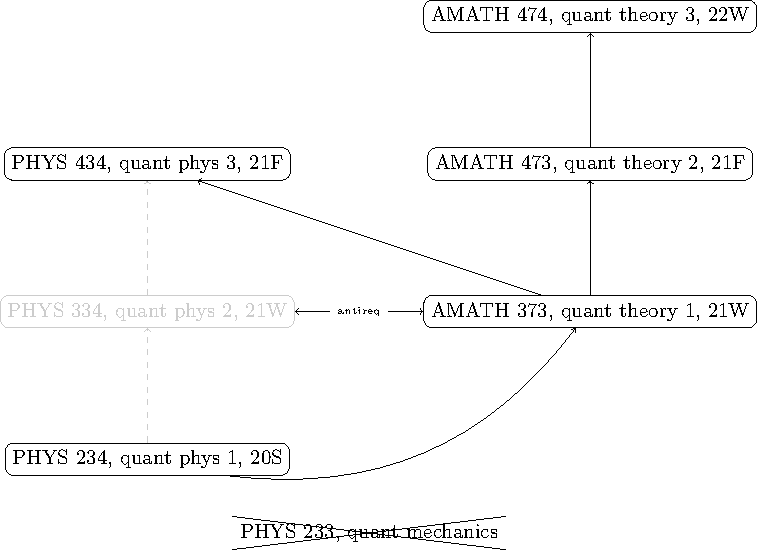
\includegraphics[width=0.95\textwidth]{../quantum/quantum}
\end{document}
